\documentclass[12pt,xcolor={table}]{beamer}
%\documentclass[12pt,xcolor={table}]{beamer}
\usetheme{Madrid}
\usecolortheme{default}


\usepackage{amsmath}
\usepackage{listings}
\usepackage{tikz}

\usetheme{default}

\title{Introduction to Algorithmic Differentiation}
\subtitle{Everything you ever wanted to know but were afraid to ask}
\author{Jean-Luc Bouchot (INRIA Saclay) \newline{} Sri Hari Krishna Narayanan (Argonne National Laboratory)}
\date{June 23, 2026}

\lstset{
  basicstyle=\ttfamily\small,
  columns=flexible,
  frame=single
}

%================================================
%= HOMEMADE COMMANDS
%================================================

% Bold face letters
\newcommand{\abf}{{\bf a}}
\newcommand{\bbf}{{\bf b}}
\newcommand{\dbf}{{\bf d}}
\newcommand{\ebf}{{\bf e}}
\newcommand{\gbf}{{\bf g}}
\newcommand{\sbf}{{\bf s}}
\newcommand{\tbf}{{\bf t}}
\newcommand{\ubf}{{\bf u}}
\newcommand{\vbf}{{\bf v}}
\newcommand{\xbf}{{\bf x}}
\newcommand{\ybf}{{\bf y}}
\newcommand{\zbf}{{\bf z}}

% Bold symbols
\newcommand{\xbs}{{\boldsymbol x}}
\newcommand{\ybs}{{\boldsymbol y}}
\newcommand{\zbs}{{\boldsymbol z}}


% Math scalar spaces
\def\Cbb{{\mathbb C}}
\def\Ebb{{\mathbb E}}
\def\Gbb{{\mathbb G}}
\def\Kbb{{\mathbb K}}
\def\Nbb{{\mathbb N}}
\def\Pbb{{\mathbb P}}
\def\Rbb{{\mathbb R}}

% Differentiation / Integration 
\newcommand{\dif}[1]{\mathrm{d} #1}

% Own colours 
\definecolor{darkerred}{RGB}{220,0,0}

\begin{document}

%================================================
\begin{frame}
\titlepage
\end{frame}

%================================================
\begin{frame}{Outline}
\tableofcontents
\end{frame}

%================================================
\section{Motivation}

%================================================
\begin{frame}{What can you expect from this tutorial?}

  Participants will:
  \begin{itemize}
    \item Understand the basics of algorithmic differentiation (AD) with respect to other approaches (finite differences, symbolic differentiation)
    \item Learn how to use AD tools for differentiating
    \item See and implement examples of forward and reverse mode AD
    \item Discuss common pitfalls and best practices for self diagnosis
    \item ... maybe even want to get involved in R \& D of AD tools!
  \end{itemize}

\end{frame}

%================================================
\begin{frame}{What we expect from you?}

  This is a diverse crowd at JDEV.
  We assume some basic understanding of the following, although we try to review the most important background material:
  \begin{itemize}
    \item Basic calculus (chain rule, partial derivatives)
    \item Basic programming (variables, loops, functions)
    \item Some familiarity with Fortran/C (but we will try to keep it as language-agnostic as possible)
    \item Some familiarity of numerical methods
    \item Some familiarity with optimization and machine learning (but not required)
  \end{itemize}

\end{frame}


%================================================
\begin{frame}{What are some successful uses of AD?}

  \begin{columns}
    \begin{column}{0.5\textwidth}
      \begin{block}{MITgcm}
        Compute XXX
      \end{block}
    \end{column}
    \begin{column}{0.5\textwidth}
      \begin{center}
        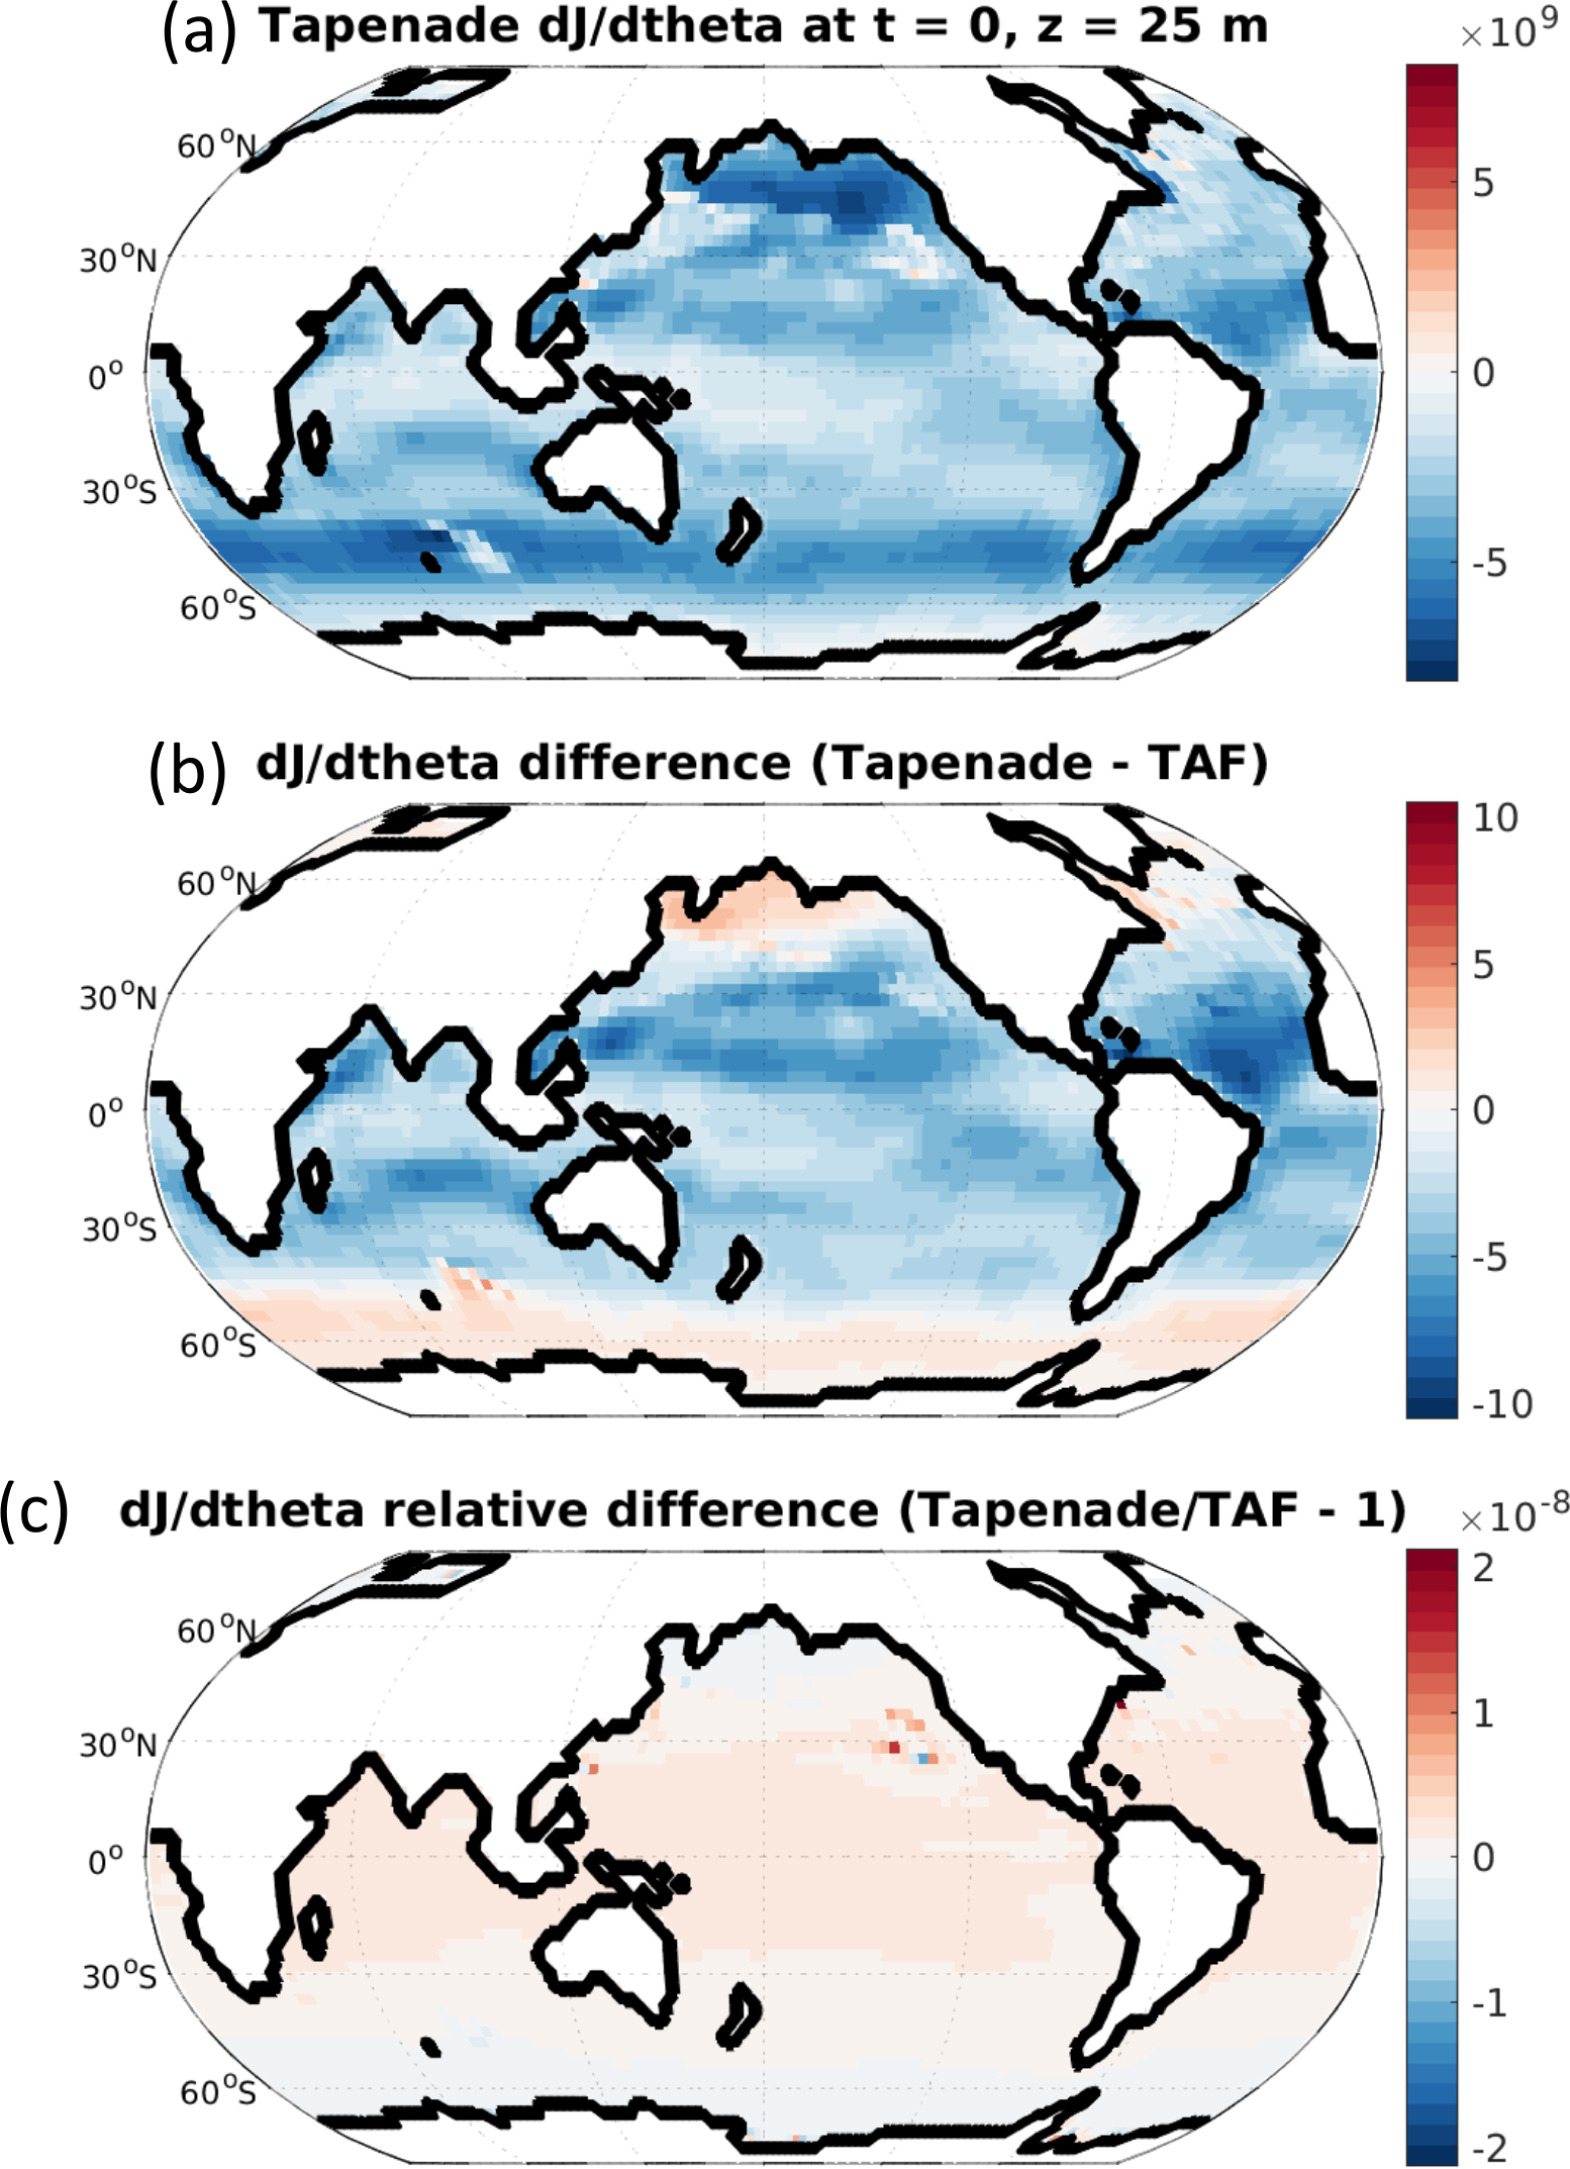
\includegraphics[width=0.8\textwidth]{FIGS/TAF-vs-TAP-mitgcm.jpg}
      \end{center}
    \end{column}
  \end{columns}


\end{frame}

%================================================
\begin{frame}{What are some successful uses of AD?}

  \begin{columns}
    \begin{column}{0.5\textwidth}
      \begin{block}{HBTHO}
        Compute XXX
      \end{block}
    \end{column}
    \begin{column}{0.5\textwidth}
      \begin{center}
        \includegraphics[width=0.8\textwidth]{FIGS/a-picture-for-hfbtho.jpg}
      \end{center}
    \end{column}
  \end{columns}


\end{frame}

%================================================
\begin{frame}{Why Do We Need Derivatives?}

Common tasks:

\begin{itemize}
\item Optimization loop
\item Sensitivity analysis
\item Data assimilation
\item Machine learning
\item PDE-constrained problems
\end{itemize}

\vspace{0.5cm}

Key question:

\begin{block}{}
How do we compute derivatives of \emph{programs} accurately and \textbf{efficiently}?
\end{block}

\end{frame}

%================================================
\section{Real valued functions}

%================================================
\begin{frame}{Three Approaches (1/3)}

\begin{block}{Finite Differences}
\begin{itemize}
\item Easy
\item Numerical error
\item Expensive in high dimension
\item Parametrization
\end{itemize}
\end{block}

\begin{block}{Example}
Let $f: \Rbb^p \to \Rbb$. Each derivative implies the computation of 
\begin{equation*}
\frac{\partial f}{\partial \xbf_i} \approx \frac{f(\xbf + \varepsilon \ebf_i) - f(\xbf [- \varepsilon \ebf_i])}{[2]\varepsilon}
\end{equation*}	
Computing the gradient costs $[2 \times] p$ the cost of a single function evaluation.
\end{block}

\end{frame}

\begin{frame}{Three Approaches (2/3)}
\begin{block}{Symbolic Differentiation}
\begin{itemize}
\item Exact
\item Expression swell
\item Hard for real codes
\end{itemize}
\end{block}

\begin{block}{Example}
Consider the function 
$f: \Rbb \to \Rbb$ defined as $f(x) = x^2\sin(x^2/2 + 3x)$. 

Its symbolic derivative is given by 
\[
\frac{\dif{f}}{\dif x} (x) = 2x\sin(x^2/2+3x) + x^2(x+3)\cos(x^2/2+3x)
\]
\end{block}

\end{frame}

\begin{frame}{Three Approaches (3/3)}
\begin{block}{Algorithmic Differentiation}
\begin{itemize}
\item Exact up to machine precision
\item Works on programs
\item Efficient
\end{itemize}
\end{block}

\begin{block}

\begin{itemize}
\item AD differentiates code, not formula!
\item AD factorizes / reuses variables
\end{itemize}

\end{block}

\end{frame}

%================================================
\section{Computational Graph View}

%================================================
\begin{frame}[fragile]{Programs as Computational Graphs}

Example:

\begin{lstlisting}
y = x1 * x2
z = sin(y)
\end{lstlisting}

\begin{center}
\begin{tikzpicture}[node distance=2cm]
\node (x1) at (0,0) {$x_1$};
%\node (x2) [below of=x1] {$x_2$};
\node (x2) at (0,2) {$x_2$};
%\node (y) [right of=x1, xshift=2cm] {$y$};
\node (y) at (2,1) {$y$};
%\node (z) [right of=y, xshift=2cm] {$z$};
\node (z) [right of=y] {$z$};

\draw[->] (x1) -- (y);
\draw[->] (x2) -- (y);
\draw[->] (y) -- (z);
\end{tikzpicture}
\end{center}

\begin{block}{Key idea}
AD = systematic application of the chain rule on this graph.
\end{block}

\end{frame}

%================================================
\begin{frame}{Differential examples}

Differenting elementary operations:

\begin{center}
\begin{tabular}{c|c|c}
Operations & Primal & Derivative \\
\hline
\texttt{add} & $z = x + y$ & $\dif{z} = \dif{x} + \dif{y}$ \\
\texttt{mul} & $z = x \times y$ & $\dif{z} = y\dif{x} + x\dif{y}$ \\
\texttt{sin} & $z = \sin(x)$ & $\dif{z} = \cos(x)\dif{x}$
\end{tabular}
\end{center}

\end{frame}

%================================================
\section{Forward Mode}

%================================================
\begin{frame}{Forward diff by dual numbers}

\begin{block}{Dual numbers}
Let every number embed its differentiated value. 
Define:

\[
\xbf^* = \xbs + \dot{\xbs}\varepsilon
\]
with the fictitious number $\varepsilon^2 = 0$.
\end{block}

$\varepsilon$ is not \emph{some small number}, but redefines the arithmetic on real numbers.

\end{frame}

\begin{frame}{Dual number propagation}

We propagate derivatives together with values.

\[
\xbf \rightarrow (\xbs, \dot{\xbs})
\]

Each operation updates both.

\pause

\begin{block}{Example}
Consider the univariate function $f(x) = x^2$.
\[
(\xbs + \dot{\xbs}\varepsilon)^2
= \xbs^2 + 2\xbs\dot{\xbs}\varepsilon \left[ + \dot{\xbs}^2 \varepsilon^2 \right].
\]

\end{block}

\begin{block}{Key insight}
Forward AD is ordinary arithmetic on dual numbers.
\end{block}

\end{frame}

%================================================
\begin{frame}{Forward Mode Example}

Given the function $z = f(x) = \sin(x^2)$

Propagation table:

\begin{center}
\begin{tabular}{c|c|c}
Variable & Value & Derivative \\
\hline
$x$ & $x$ & $\dot{x}$ \\
$y=x^2$ & $x^2$ & $2x\dot{x}$ \\
$z=\sin(y)$ & $\sin(y)$ & $\cos(y)\cdot 2x\dot{x}$
\end{tabular}
\end{center}

\begin{block}{Let's try}
\begin{itemize}
\item $f(x) = \sin(x)$
\item $f(x) = \cos(x)$
\item $f(x) = \sqrt{x}$
\end{itemize}
\end{block}

\end{frame}

\begin{frame}{Let's try}
  \begin{block}{$\sin$}
    \vspace{-0.5cm}
    \begin{align*}
      \sin(x + \dot{x}\varepsilon) &= \sin(x)\cos(\dot{x}\varepsilon) + \cos(x)\sin(\dot{x}\varepsilon) \\
      &= \sin(x)\left( 1 + \mathcal{O}(\dot{x}^2\varepsilon^2) \right) + \cos(x)(\dot{x}\varepsilon + \mathcal{O}(\dot{x}^3\varepsilon^3)) \\
      &= \sin(x) + \cos(x)\dot{x}\varepsilon
    \end{align*}
  \end{block}

  \begin{block}{$\cos$}
    \vspace{-0.5cm}
    \begin{align*}
      \cos(x + \dot{x}\varepsilon) &= \cos(x)\cos(\dot{x}\varepsilon) - \sin(x)\sin(\dot{x}\varepsilon) \\
      &= \cos(x)\left( 1 + \mathcal{O}(\dot{x}^2\varepsilon^2) \right) - \sin(x)(\dot{x}\varepsilon + \mathcal{O}(\dot{x}^3\varepsilon^3)) \\
      &= \cos(x) - \sin(x)\dot{x}\varepsilon
    \end{align*}
  \end{block}

  \begin{block}{$\sqrt{\cdot}$}
    \vspace{-0.5cm}
    \begin{align*}
      \sqrt{x + \dot{x}\varepsilon} &= \sqrt{x}\sqrt{1 + \frac{\dot{x}}{x}\varepsilon}
      &= \sqrt{x}\left( 1 + \frac{1}{2}\frac{\dot{x}}{x}\varepsilon + \mathcal{O}(\dot{x}^2\varepsilon^2) \right) \\
      &= \sqrt{x} + \frac{\dot{x}}{2\sqrt{x}}\varepsilon
    \end{align*}
  \end{block}
\end{frame}

%================================================
\begin{frame}{Forward Mode review}

\begin{block}{Idea}
Forward AD propagates perturbations: "How much is this output influenced by a small change in this input?"
\end{block}

\begin{block}{Rule of thumb}
Cost $\propto$ number of inputs
\end{block}

Best when:

\begin{itemize}
\item Few inputs
\item Many outputs
\end{itemize}

\end{frame}

\begin{frame}{Left to right or right to left}

A program computes {\bf out} from {\bf in}:
\begin{equation*}
{\textbf{in}} \rightarrow {\tt v_1} \rightarrow {\tt v_2} \rightarrow \cdots \rightarrow {\tt v_9} \rightarrow {\textbf{out}}
\end{equation*}
One can propagate ${\dif{\tt v}\over \dif{\bf in}}$ forward $\Rightarrow$ Tangent (JVP, more later):
\begin{equation*}
{\color{red}1.0} = \dot{\textbf{in}} = \frac{\dif{\textbf{in}}}{\dif{\textbf{in}}} \rightarrow \frac{\dif{\tt v_1}}{\dif{\textbf{in}}} \rightarrow\frac{\dif{\tt v_2}}{d\textbf{in}} \rightarrow \cdots \rightarrow \frac{\dif{\tt v_9}}{\dif\textbf{in}} \rightarrow \frac{\dif{\textbf{out}}}{\dif{\textbf{in}}}
\end{equation*}
One can propagate ${\dif{\bf out}\over \dif{\tt v}}$ backward $\Rightarrow$ Adjoint (VJP, more later):
\begin{equation*}
\frac{{\dif{\textbf{out}}}}{\dif{\textbf{in}}} \leftarrow \frac{\dif{\textbf{out}}}{\dif{\tt v_1}} \leftarrow \frac{\dif{\textbf{out}}}{\dif{\tt v_2}} \leftarrow \cdots \leftarrow \frac{{\dif\textbf{out}}}{\dif{\tt v_9}} \leftarrow \frac{\dif{\textbf{out}}}{\dif{\textbf{out}}} = \bar{\textbf{out}}{\color{red}1.0}
\end{equation*}
The {\color{red} initialization} are called {\color{red} seeds} when dealing with many variables.
\end{frame}

\begin{frame}{Costs of Tangent and Adjoint AD}
$f \>\>:\>\>\>\> \hbox{\bf in} \in \Rbb^{p} \>\>\rightarrow\>\> \hbox{\bf out} \in \Rbb^{n}$, computed with cost ${\tt P}$\\
\centerline{}
\begin{minipage}[c]{20mm}
{${{\bf d\>out}\over {\bf d\>in}} = $}
\end{minipage}
\begin{minipage}[c]{60mm}
%{\includegraphics[width=8cm, height=3.5cm]{FIGURES/costMatrix}}
\begin{equation*}
  \left(\begin{array}{cccc>{\columncolor{olive!20}}cc}
    * & * & * & * & * & * \\
    \rowcolor{red!20}
    * & * & * & * & * & * \\
    * & * & * & * & * & * \\
    * & * & * & * & * & * 
  \end{array}\right)
\end{equation*}
\end{minipage}
\centerline{}
\begin{itemize}
\item ${\bf d\>out}\over {\bf d\>in}$ costs {\color{darkerred}$p*4?*{\tt P}$} using the {\color{olive}tangent mode}\\
      \indent Good if $n > = p$
\item ${\bf d\>out}\over {\bf d\>in}$ costs {\color{darkerred}$n*4?*{\tt P}$} using the {\color{red}adjoint mode}\\
      \indent Good if $n \ll p$ (e.g $n=1$ for a gradient)
\end{itemize}
\end{frame}

%================================================
\section{Multivalued inputs or outputs}

\begin{frame}{Differentiating non high school functions}
  A function $F = f_p \circ f_{p-1} \circ \cdots \circ f_1: \mathbb{R}^n\to\mathbb{R}^d$ is implemented through a program  \newline{}
  
  {\begin{center} \texttt{P: \{ I\_1, I\_2, \dots, I\_p \}} \end{center}}

  Defining $V_0 = \texttt{\textbf{in}}$ and $V_k = f_k(V_{k-1})$


\end{frame}

%================================================

%================================================
\section{Reverse Mode}

%================================================

\begin{frame}{Reverse Mode Goal}

We want gradients in high dimensional input spaces:

\[
f:\mathbb{R}^p \to \mathbb{R}
\]

\pause

\begin{block}{Idea}
\begin{itemize}
\item Accumulate variations from the output
\item Propagate \emph{sensitivities} backwards
\end{itemize}
\end{block}

\end{frame}

%================================================
\begin{frame}{Adjoint Variables}

Define for each variable $v$:

\[
\bar{v} = \frac{\partial z}{\partial v}
\]

Initialize:

\[
\bar{z} = 1
\]

\end{frame}

%================================================
\begin{frame}[fragile]{The Aha Moment: Why += ?}

Consider:

\begin{lstlisting}
y = x*x
z = y + y
\end{lstlisting}

\pause

Derivative:

\[
\frac{\partial z}{\partial y} = 2
\]

\pause

Backward propagation:

\begin{align*}
\bar{y} &+= 1 \\
\bar{y} &+= 1
\end{align*}

\begin{block}{Key message}
Adjoints accumulate because multiple paths contribute.
\end{block}

\end{frame}

%================================================
\begin{frame}{General Reverse Rule}

For any variable $v$:

\[
\bar{v} = \sum_{w\in children(v)}
\bar{w}\frac{\partial w}{\partial v}
\]

\begin{block}{Interpretation}
Reverse mode sums contributions from all downstream paths.
\end{block}

\end{frame}

%================================================
\begin{frame}{Cost of Reverse Mode}

\begin{block}{Rule of thumb}
Cost $\propto$ number of outputs
\end{block}

Best when:

\begin{itemize}
\item Many inputs
\item Scalar output
\end{itemize}

\end{frame}

%================================================
\section{Pitfalls}

%================================================
\begin{frame}{Common Pitfalls}

\begin{itemize}
\item Non-differentiable functions (abs, max)
\item Hidden state
\item Memory in reverse mode
\item Aliasing in Fortran
\end{itemize}

\end{frame}

%================================================
\section{Summary}

%================================================
\begin{frame}{Takeaways}

\begin{itemize}
\item AD applies the chain rule to programs
\item Forward mode: push derivatives
\item Reverse mode: pull sensitivities
\item Reverse requires accumulation (+=)
\item Tapenade automates the process
\end{itemize}

\end{frame}

%================================================
\begin{frame}
\centering
\Huge Now let's get started!
\end{frame}

%================================================
\section{Tapenade Practice}

%================================================
\begin{frame}[fragile]{Example Fortran Code}

\begin{lstlisting}
double precision function energy(x)
double precision x
energy = x*x + sin(x)
end
\end{lstlisting}

\end{frame}

%================================================
\begin{frame}[fragile]{Running Tapenade}

Forward mode:

\begin{lstlisting}
tapenade -forward -head energy energy.f
\end{lstlisting}

Reverse mode:

\begin{lstlisting}
tapenade -reverse -head energy energy.f
\end{lstlisting}

\end{frame}

%================================================
\begin{frame}{What Tapenade Generates}

You will see:

\begin{itemize}
\item Tangent variables (forward)
\item Adjoint variables (reverse)
\item Two-pass structure in reverse mode
\end{itemize}

\end{frame}

%================================================
\begin{frame}[fragile]{Loop Example}

\begin{lstlisting}
do i = 1, n
   y = y + a(i)*x(i)
end do
\end{lstlisting}

\begin{block}{Important}
AD differentiates through loops automatically.
\end{block}

\end{frame}

\end{document}